\section*{Test 11 Choice of escape route}

A public space has 2 exits: exit 1 and exit 2. Choose a population of adults from Figure 5 with an immediate reaction and distribute the walking speeds over a population of 1,000 persons. The space should be occupied from the left side with the maximum possible density. The expected result is that the persons prefer the closer exit 1 and congestion occurs in this area. However, individual persons will also use the alternative exit 2.

\begin{figure}[h]
	\centering
	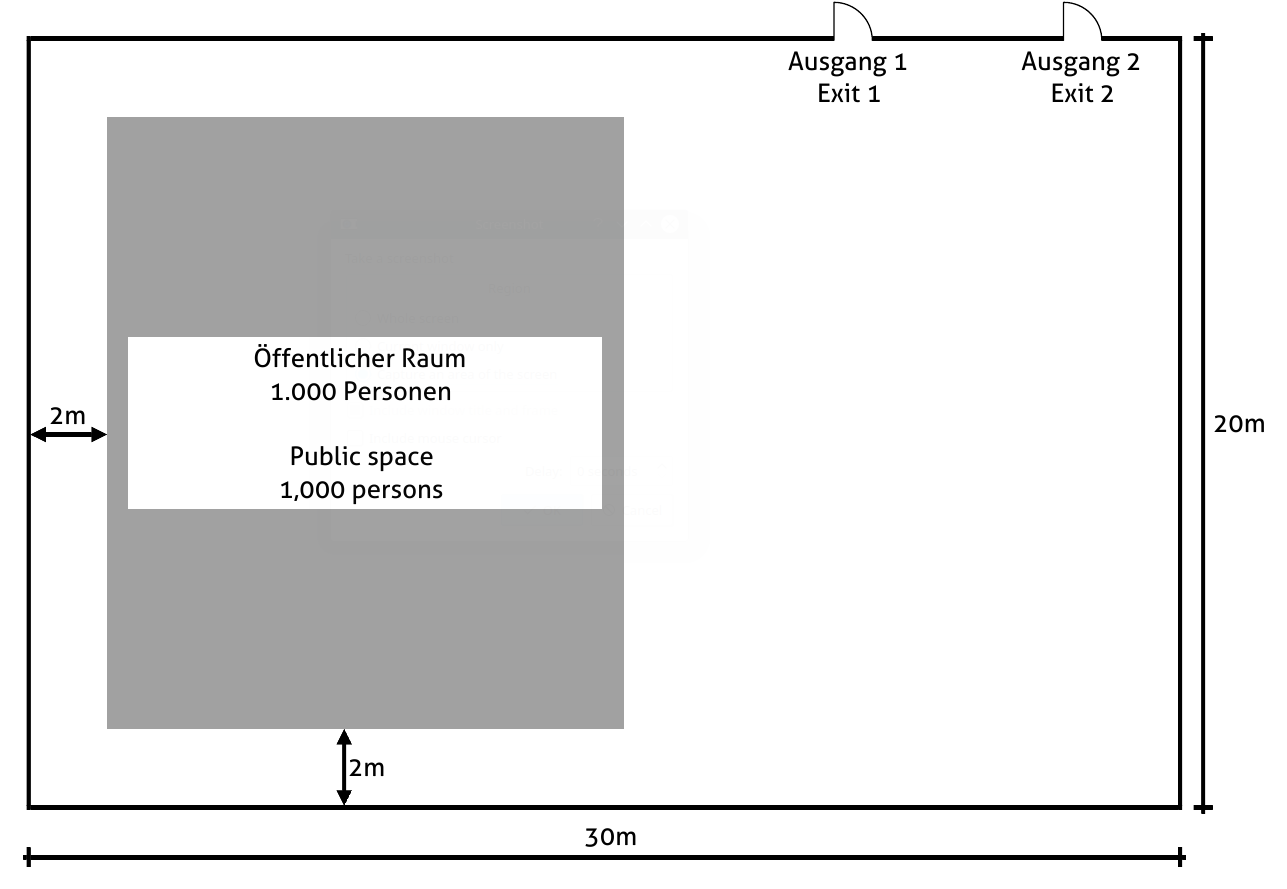
\includegraphics[scale=0.44]{test_description/Large_public_space_test_11.png}
	\caption{\footnotesize \textbf{Leavin a space vis two exits}}
\end{figure}
